\documentclass[margin=10pt]{standalone}    

\usepackage{tikz}
\usetikzlibrary{automata, positioning, arrows}

\begin{document}

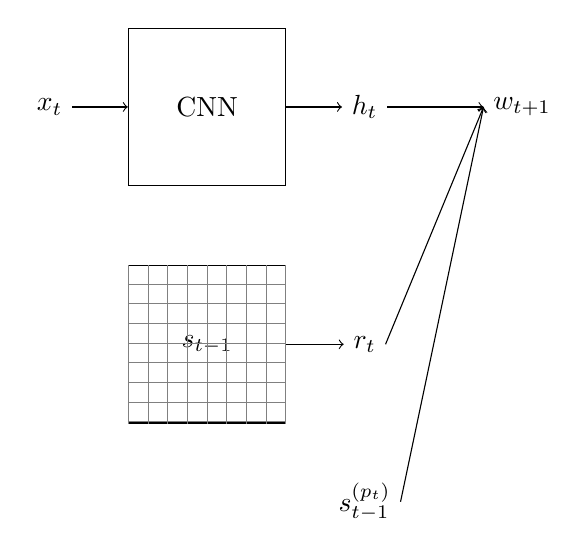
\begin{tikzpicture}[node distance=2cm]
    \tikzstyle{block} = [rectangle,minimum width=2cm,minimum height=2cm,text centered,draw=black,fill=white]
        
    \node (cnn) [block]{CNN};
    
    \node (map) [block, below=1cm of cnn] {$s_{t-1}$};
    \draw [step=0.25,gray,thin] (map.north west) grid (map.south east);

    \node (x) [left of=cnn]{$x_t$};
    
    \node (h) [right of=cnn]{$h_t$};
    \node (r) [right of=map]{$r_t$};
    \node (m) [below of=r]{$s_{t-1}^{(p_t)}$};

    \node (w) [right of=h]{$w_{t+1}$};

    \draw [->] (x.east) -- (cnn.west);

    \draw [->] (cnn.east) -- (h.west);
    \draw [->] (map.east) -- (r.west);

    \draw [->] (h.east) -- (w.west);
    \draw [->] (r.east) -- (w.west);
    \draw [->] (m.east) -- (w.west);

    %\draw [->] (p.north) -- (map.south);
    %\draw [->] (cnn.east) -- node[anchor=south]{$h_t$} (map.west); 
    %\draw  (map) edge[loop above] (map);
\end{tikzpicture}

\end{document}
